% !TEX TS-program = pdflatex
\documentclass[12pt]{report}

% Package the packages
\usepackage[T1]{fontenc}
\usepackage[utf8]{inputenc}
\usepackage{lmodern}
\usepackage[a4paper, margin=0.75in]{geometry}
\usepackage{enumitem}
\usepackage[colorlinks=true, linkcolor=black, citecolor=black, urlcolor=blue]{hyperref}
\usepackage[nottoc,numbib]{tocbibind}
\usepackage[round]{natbib}
\usepackage{pdfpages}
\usepackage{fancyvrb}
\usepackage[parfill]{parskip}
\usepackage{titlesec}
\usepackage{listings}
% -

% Configuration
% Change font to Palatino
\renewcommand{\rmdefault}{ppl}
% Change the list item spacing
\setlist{noitemsep}
% Set the bibliography style
\bibliographystyle{usw}
% Set up a terminal command block
\definecolor{light-gray}{gray}{0.95}
\newcommand{\term}[1]{\colorbox{light-gray}{\texttt{#1}}}
% Set up better chapter titling
\titleformat{\chapter}{\normalfont\LARGE\bfseries}{\thechapter.}{12pt}{}
\titlespacing{\chapter}{0pt}{0pt}{12pt}
\titleformat{\section}{\normalfont\Large\bfseries}{\thesection}{12pt}{}
\titlespacing{\section}{0pt}{0pt}{6pt}
\titleformat{name=\section,numberless}{\normalfont\Large\bfseries}{}{0pt}{}
\titleformat{\subsection}{\normalfont\large\bfseries}{\thesubsection}{12pt}{}
\titleformat{name=\subsection,numberless}{\normalfont\large\bfseries}{}{0pt}{}
\titlespacing{\subsection}{0pt}{0pt}{3pt}
% -

% Definitions
\title{IY1D402\thanks{University of South Wales, National Cyber Security Academy}\\{\textit{\small Cyber Security Tools And Practices}}\\Assessment 1 Remote Exploitation Report}
\author{David Sanders\\{\LARGE 17135397}}
\date{\today}
% -

% Document
\begin{document}

% Cover page setup
\maketitle
\pagebreak
% 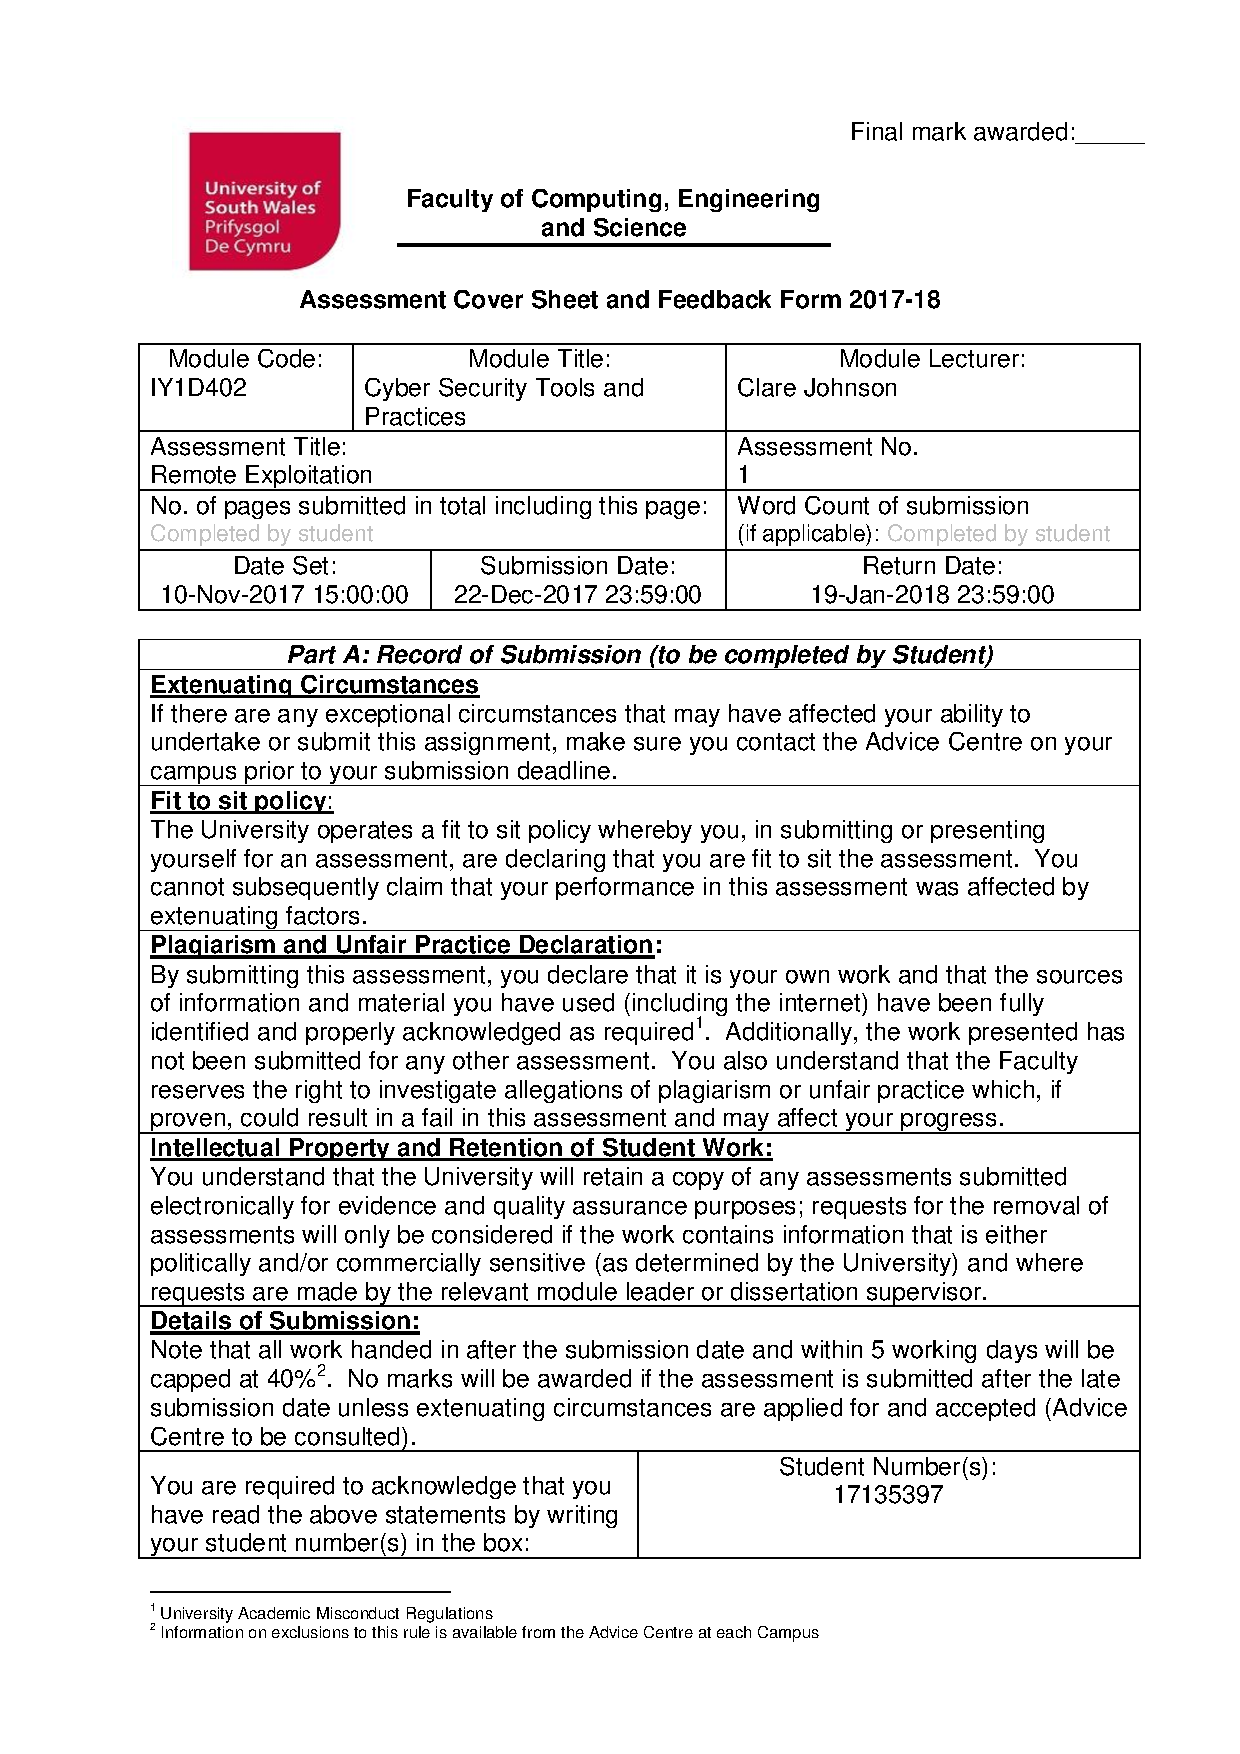
\includepdf[pages={1}]{assignmentbrief/IY1D402_CW1M_Cover_PRO_PROJECT1.pdf}
\tableofcontents
% -

% Introduction
\pagebreak
\chapter{Introduction}
For the first formal assessment of our IY1D402 \textit{(Cyber Security Tools and Practices)} we have been given a real-world scenario. We have been asked to, individually, conduct an investigation before writing a report that details the methodology that we followed during our investigation, presents our findings, discusses the capabilities of the tools we used, describes alternative methods that could have been used, and explains the nature of \textit{'insider threat'}. The target audience is a Senior Management Team and so, although it is a technical, this report will attempt to present technical aspects with enough explanation to make them understandable by those who are not technical specialists.

\section{Scenario}
I am the Senior Technical Officer at eCorp and have been asked by the Senior Management Team to investigate an employee -- Phillip Price -- who is suspected of exfiltrating Intellectual Property (IP) from the company.

To verify this suspicion, I have been asked to monitor Price's activities on the company's IT system, and have been given permission to use any appropriate methods in the course of this investigation. It has also been requested that I take suitable steps to conceal this monitoring from Price.

Upon completion of the investigation, I have been asked to write a report for the Senior Management Team that details exactly the steps that I took and explains my findings. I should also discuss the capabilities of the tools that I used and explain whether any alternative methods could have been used at various stages of the investigation.

Finally, to complete the report, I should explain the nature of \textit{'insider threat'} and its implications to an organisation while giving examples of where such threats have occurred in the past, discussing how the tools that I used impact on the organisation's security, and suggesting methods for improving our security in the future.

To aid in my investigation, I have been provided with a list of commonly used passwords that might help me to gain access to Price's machine.
% -


% Glossary
% \pagebreak
% \chapter{Glossary}
% todo: Maybe add a glossary - one would probably included in this sort of technical report (that is, one with a not necessarily technical audience)
% -


% Preliminary Report
\pagebreak
\chapter{Preliminary Report}
During the investigation, I gathered a lot of information regarding Price's machine and account. I will summarise the most important points in a table below and detail fully the methodology by which I acquired this information in the next chapter of the report.

\begin{table}[h!]
  \centering
  \begin{tabular}{|r l|}
    % \hline
    % \multicolumn{2}{||l||}{Information} \\
    % \hline\hline
    \hline
    IP address: & 192.168.254.132 \\
    \hline
    Operating system: & Linux Ubuntu 4.13.0-17-generic x86\_64 \\
    \hline
    % Open Ports\footnotemark : & [details the ports] \\
    Open ports: & 80 \textit{[http]}, 442 \textit{[ssh; OpenSSH 7.5p1 Ubuntu 10]} \\
    \hline
    Closed ports: & 443 \textit{[https]} \\
    \hline
    Price's groups: & phillip adm cdrom sudo dip www-data plugdev lpadmin sambashare \\
    \hline
  \end{tabular}
  \caption{Information on Price's machine and account}
  \label{table:pricemachineinfo}
\end{table}
% \footnotetext{Common and in-range 1-1000}

The IP address was found by scanning the network with \texttt{arp-scan} and the ports were found using \texttt{Nmap}

While logged in via SSH to Price's machine, the OS was found using \term{uname -a} and Price's groups with \term{groups}
% -


% Investigate Methodology
\pagebreak
\chapter{Investigative Methodology}
In this section of the report, I will describe in detail the steps that I took to find, gain access to, and monitor Price's machine during the investigation. In order to keep this section of the report as concise as possible, I have included evidential deliverables (screenshots and code) of some of the steps in the process in the appendices.


\section*{Setting up the Virtual Machines}
Due to the way in which the hypothetical scenario was presented, I had to set up two virtual machines in VMWare Workstation in order to conduct the analysis of the Price's machine. In reality, Price's machine would most likely be a physical computer connected to the eCorp network.

Firstly, I set up a new VM \textit{('IY1D402 A1;2 (ECORP; 20171117)')} using the VMDK (Virtual Machine Disk) image of Price's machine that we had been provided. I configured the network adaptor in this machine to connect to a host-only network, which was provided by the VMWare software.

Secondly, I configured my existing attack VM \textit{('It's Elementary my dear Watson!')} to have two network adaptors - the existing NAT adaptor, which allows it to connect to the Internet, and the host-only network adaptor.

After completing this steps, I \textit{'powered on'} both of the virtual machines.


\section{Searching the network}
The first stage of investigation is to find the IP address of Price's machine on the network -- in the real world, this IP would likely be provided to us by the network administrator. However, even though it would be harder to do in a network with more than two machines, I will describe how I used \texttt{ifconfig} and \texttt{arp-scan} to find the IP address.

\subsection{Using \texttt{ifconfig} to find the host-only network interface name}
In order to be able to use \texttt{arp-scan} in the second part of this stage, I needed to know the interface name of the host-only network on the attack VM. To find the interface name I used the \term{ifconfig} command.

As I knew that the NAT adaptor interface is called \textit{ens33}, the relevant output of this command is:
\begin{Verbatim}[frame=leftline]
ens34     Link encap:Ethernet  HWaddr 00:0c:29:72:88:f2
          inet addr:192.168.254.135  Bcast:192.168.254.255  Mask:255.255.255.0
          inet6 addr: fe80::490:c374:f983:b700/64 Scope:Link
          UP BROADCAST RUNNING MULTICAST  MTU:1500  Metric:1
          RX packets:52792 errors:0 dropped:0 overruns:0 frame:0
          TX packets:56528 errors:0 dropped:0 overruns:0 carrier:0
          collisions:0 txqueuelen:1000
          RX bytes:9729912 (9.7 MB)  TX bytes:10084091 (10.0 MB)
\end{Verbatim}

From this, I could discern that the host-only interface name is \textit{ens34}.

\subsection{Using \texttt{arp-scan} to find the IP address of Price's machine}
In order to discover the IP addresses of machines in the network I used the command:\\
\term{sudo arp-scan -lI ens34}

The output of this command was:
\begin{Verbatim}[frame=leftline, fontsize=\small]
Interface: ens34, datalink type: EN10MB (Ethernet)
Starting arp-scan 1.8.1 with 256 hosts (http://www.nta-monitor.com/tools/arp-scan/)
192.168.254.1	00:50:56:c0:00:01	VMware, Inc.
192.168.254.132	00:0c:29:e2:a5:34	VMware, Inc.
192.168.254.254	00:50:56:ed:f1:b4	VMware, Inc.

3 packets received by filter, 0 packets dropped by kernel
Ending arp-scan 1.8.1: 256 hosts scanned in 1.342 seconds (190.76 hosts/sec). 3 responded
\end{Verbatim}

As my attack machine IP is not shown and 192.168.254.1/254 are \textit{services} operated by VMWare to support the operation of the host-only network, I could see that \textbf{192.168.254.132} must be the IP address of the Price's machine.


\section{Scanning Price's machine}
With the IP address of Price's machine, I used Nmap to scan the machine for open ports and find the SSH service.
\subsection{Running a basic \texttt{nmap} scan}
Initially, I ran a basic Nmap scan using:\\
\term{sudo nmap 192.168.254.132}

The result of this scan was:
\begin{Verbatim}[frame=leftline]
Starting Nmap 7.01 ( https://nmap.org ) at 2017-12-06 13:31 GMT
Nmap scan report for 192.168.254.132
Host is up (0.00045s latency).
Not shown: 998 filtered ports
PORT    STATE  SERVICE
80/tcp  open   http
443/tcp closed https
MAC Address: 00:0C:29:E2:A5:34 (VMware)

Nmap done: 1 IP address (1 host up) scanned in 17.56 seconds
\end{Verbatim}

From this scan, I could see that port 80 was open and port 443 was closed. Connecting to the machine with a browser brought up a web page and so I could tell that the machine is definitely serving http requests on port 80. I did not find the SSH port in this scan and so it must have been moved from the port 22 (the default) to a different port.

\subsection{Expanding the \texttt{nmap} scan to find the SSH port}
In order to try and find the SSH port without having to run a complete scan of all 65535 ports, I decided to run a scan of ports 1-1000 to see if the SSH service had been moved to a port in this range. To do this, I used the command:\\
\term{sudo nmap -p 1-1000 192.168.254.132}

The result of this command was:
\begin{Verbatim}[frame=leftline]
Starting Nmap 7.01 ( https://nmap.org ) at 2017-12-06 13:34 GMT
Nmap scan report for 192.168.254.132
Host is up (0.00045s latency).
Not shown: 997 filtered ports
PORT    STATE  SERVICE
80/tcp  open   http
442/tcp open   cvc_hostd
443/tcp closed https
MAC Address: 00:0C:29:E2:A5:34 (VMware)

Nmap done: 1 IP address (1 host up) scanned in 14.16 seconds
\end{Verbatim}

This scan revealed that there was a service running on open port 442. Although Nmap identifies this service as \textit{cvc\_hostd}, the service identification method used in basic Nmap scans only uses port number to guess the service.

\subsection{Using \texttt{nmap} service detection to confirm the SSH port}
I used service detection to see if the SSH port had been moved to port 442. To do this, I used the command:\\
\term{sudo nmap -sV -p 442 192.168.254.132}

The result of this command was:
\begin{Verbatim}[frame=leftline]
Starting Nmap 7.01 ( https://nmap.org ) at 2017-12-06 13:38 GMT
Nmap scan report for 192.168.254.132
Host is up (0.00041s latency).
PORT    STATE SERVICE VERSION
442/tcp open  ssh     OpenSSH 7.5p1 Ubuntu 10 (Ubuntu Linux; protocol 2.0)
MAC Address: 00:0C:29:E2:A5:34 (VMware)
Service Info: OS: Linux; CPE: cpe:/o:linux:linux_kernel

Service detection performed.
Please report any incorrect results at https://nmap.org/submit/ .
Nmap done: 1 IP address (1 host up) scanned in 1.20 seconds
\end{Verbatim}

This command asked Nmap to attempt to do service detection against only port 442 on 192.168.254.132 and the result shows that the SSH service \textit{[version: OpenSSH 7.5p1 Ubuntu 10 (Ubuntu Linux; protocol 2.0)]} had been moved to this port.


\section{Breaking into Price's account}
Having discovered the SSH service port, I decided to try and break into Price's account via SSH using the list of passwords provided to me. Doing this manually by hand would be an time-consuming and arduous task individually and so I decided to write a script in Python to automate this attack.

Using Python 3 and pexpect \textit{(a library for handling SSH connections)}, I wrote a script that:
\begin{enumerate}
  \item Loads the passwords from the wordlist provided
  \item Sets up a pool of processes to run tasks - using a pool is faster than attempting each password in series
  \item Creates a connection attempt task for each password and passes the task to the pool for processing
  \item Collects the results from finished tasks and checks to see if the task found the correct password
  \item If the correct password is found, the pool is terminated to prevent further processing and the script finishes after performing a basic reconnaissance stage over the SSH
\end{enumerate}

The full code listing for the script can be found in Appendix~\ref{app:code:sshcrack_mp}.

To attack Price's SSH account \textit{('phillip')} at the IP address 192.168.254.132 on port 442 with the wordlist \textit{('passwords.txt')}, the script can run using:\\
\term{./sshcrack\_mp.py phillip:192.168.254.132:442 passwords.txt}\footnote{Usage in this way requires a virtual environment in \texttt{venv} with the pexpect dependency installed in it}

The output, with a section of the failed password attempts removed for brevity, is:
\begin{Verbatim}[frame=leftline]
Loaded 393 passwords from 'passwords.txt'
(001/393; 00.25%) Password != '0'
(002/393; 00.51%) Password != 'scorpio'
(003/393; 00.76%) Password != 'buddy'
...
(222/393; 56.49%) Password != 'trustno1'
(223/393; 56.74%) Password != 'newyork'
(224/393; 57.00%) Password == 'qwertyuiop'
Took 0.96 minutes to check 224/393 passwords at a rate of 3.88pw/s.
Performing recon...
Logging out.
\end{Verbatim}

From the output above, I could see that the script successfully broke into Price's SSH account using the password: \texttt{qwertyuiop}


\section{Examining Price's account}
A reconnaissance phase is performed automatically as the last step in the script used to break into Price's SSH account. In this stage, the script calls a couple of commands over the SSH connection and writes the results into a \texttt{recon.txt} file on the attack machine. A copy of this file is included in Appendix~\ref{app:files:recon} -- included in this is a \term{cat} of the \texttt{/etc/passwd} file.

I could see from the \texttt{recon.txt} file that Price is a member of the sudo group. This made the rest of the investigation easier to conceal as I could wipe/modify logs and create new users in order to keep the investigation concealed.

Using the password discovered in the previous step of the investigation, I logged into Price's account via SSH to examine it and the machine remotely, and to gather more intelligence. [see screenshot proving log in and intel gathering] The command that I used to connect over SSH was:\\
\term{ssh -p 442 phillip@192.168.254.132}

I also used \texttt{scp} to pull a copy of the \texttt{/var/log/auth.log} from Price's machine -- it is attached, in a reduced form, in Appendix~\ref{app:files:authlog}. To do this, I used the command:\\
\term{scp -P 442 phillip@192.168.254.132:/var/log/auth.log auth.log}

In this log file, I can see a lot of evidence of failed attempts to log into Price's SSH account on the machine before the correct password is found and authentication is successful -- I will need to remove or modify this file to conceal the investigation from Price.


\section{Setting up persistent access to the machine}
In order to maintain persistent access to Price's machine I decided to create a new user with the command:\\
\term{sudo adduser systemd-usertest}

I used the username \textit{'systemd-usertest'} in an effort to disguise my presence from Price. As systemd provides a myriad of services, Price would hopefully attribute this new user to a \texttt{systemd} update.

After creating the \textit{'systemd-usertest'} user, I made it a member of the \texttt{sudo} group with the command:\\
\term{sudo usermod -aG sudo systemd-usertest}

With this new account, I was able and will continue to be able to access Price's machine on demand for the course of the investigation.

The screenshot in Appendix [blahref] shows me accessing this new account over SSH from my attack machine.


\section{Setting up a \texttt{squid} proxy to monitor traffic}
\subsection{Setting up \texttt{squid} on the attack machine}
In order to monitor Price's web traffic I set up a \texttt{squid} proxy on my attack machine. I did this using the following commands:
\begin{enumerate}
  \item Install \texttt{squid} with:\\
        \term{sudo apt install squid}
  \item Open the \texttt{squid.conf} file for editing by using:\\
        \term{sudo vim /etc/squid/squid.conf}
  \item In the relevant section of the configuration file, define a new ACL that defines a source and IP address range with:\\
        \term{acl monitornet src 192.168.254.0/24}
  \item In the relevant section of the configuration file, define a \texttt{http\_access} rule that allows \textit{monitornet} with:\\
        \term{http\_access allow monitornet}
  \item If ufw (firewall) is active, allow connections to port 3128 from relevant IP addresses with:\\
        \term{sudo ufw allow from 192.168.254.0/24 to any port 3128}
\end{enumerate}

\subsection{Setting up Price's machine to use the proxy}
% I could have configured Price's machine to use the proxy by entering the IP address and \texttt{squid} port into the proxy settings in Firefox. However, it would be easy for Price to see that a change had been made if he checked the proxy settings.
%
% Instead, I decided to configure the machine to use the proxy at the system level by using, via SSH to Price's machine, the commands:
% \begin{itemize}
%   \item \term{}
% \end{itemize}


\subsection{Proving with \texttt{wireshark} that the proxy is working}



\section{Concealing the investigation from Price}
todo: discuss steps that I took to conceal the investigation from Price, and detail some further methods that I could have taken

Steps could include:
\begin{enumerate}
  \item Wiping the \texttt{/var/log/auth.log} or modifying it (and it's compressed older copies) to remove the ssh login attempt lines
  \item Clearing the bash history
  \item Clearing any SSH specific logs
  \item Using uptime to check that I am the only user of the machine upon SSH login -- as in, Price is not also using the machine
\end{enumerate}


\pagebreak
\chapter{Tool Capabilities and Alternative Methods}
In this section, I will discuss briefly the capabilities of the tools I used in this investigation and also provide examples of alternative tools/methods that could have used to similar effect.

\section{\texttt{arp-scan}}
\texttt{arp-scan} is a command-line tool for system discovery and fingerprinting.\footnote{http://www.nta-monitor.com/wiki/index.php/Arp-scan\_User\_Guide} By constructing and sending ARP \textit{(Address Resolution Protocol)} requests to specified IP addresses, it can be used to discover hosts connected to a local IP network. The ARP protocol determines the link-layer (layer 2) address for a specified network-layer (layer 3) address. It can be used to discover all hosts, including those blocking traffic with firewalls. Although designed to be used for any link-layer and network-layer protocols, in practice it is only used for IPv4 Ethernet and 802.11 wireless traffic. IPv6 uses a different protocol called NDP \textit{(Network Discovery Protocol)}.

In the investigation, \texttt{arp-scan} was used to discover the IP address of Price's machine.
\subsection*{Alternative Tools/Methods}
\texttt{nmap} can also be used to perform network discovery.
% with the command:\\
% \term{todo: put command here}

\section{\texttt{nmap}}
\texttt{nmap} \textit{("Network Mapper")} is an open source tool for network exploration and security auditing.\footnote{https://nmap.org/book/man.html} Although it can be used to scan individual hosts, it was designed to allow large networks to be scanned rapidly. \texttt{nmap} is capable of determining the available hosts on a network, the services that these hosts are providing, the operating systems that they are running, the type of packet filters/firewalls that are in use, and other characteristics. As well as being used for security audits, it can also be useful for routine system/network administration tasks such as inventorying the network, service upgrade schedule management, and monitoring host/service uptime.
\subsection*{Alternative Tools/Methods}
Although alternative tools do exist, \texttt{nmap} is arguably the most complete and well-supported network scanning tool. It was originally released in September 1997 but the latest stable release was on 31\textsuperscript{st} July 2017.

\section{\texttt{python}}
Python\footnote{https://www.python.org/} is a high-level scripted programming language that supports multiple paradigms: object-oriented, imperative, functional, procedural, and reflective. Though first released in 1991, the latest version (3.6.3) was released on 3\textsuperscript{rd} October 2017.

With a substantial standard library and a plethora of third-party libraries (such as pexpect) available, it is highly suited for use as a programming language to develop both small scripts, for automation of tasks; and larger programs, which could include GUIs (Graphical User Interfaces).

As Python combines a dynamic type system and automatic memory management with a design philosophy that emphasises code readability\footnote{As long as you follow the PEP8 recommendations}, it is quite easy to learn for beginners and highly suited for quickly prototyping ideas in the hands of more experienced developers.

The reference implementation of Python, \textit{CPython}, is open source software.
\subsection*{Alternative Tools/Methods}
Almost any other programming language could have been used for the investigation in lieu of Python. As long as a library, for that language, exists that allows it to make SSH connections, or the language is capable of calling other programs \textit{('ssh')} on the machine, it would be possible to create an equivalent SSH cracking script.

\section{\texttt{squid}}
Squid\footnote{http://www.squid-cache.org/} is a web proxy that provides caching and forwarding services. Squid includes some support for protocols such as Internet Gopher, SSL, TLS, and HTTPS but is mainly used for HTTP and FTP traffic. During the investigation Squid was used to filter and monitor traffic but it can also be used to speed up traffic by caching web, DNS, and other lookup traffic for those sharing network resources.
\subsection*{Alternative Tools/Methods}
There a lot of different forwarding proxies that could have been used in place of Squid, such as \href{https://docs.trafficserver.apache.org/en/5.3.x/admin/forward-proxy.en.html}{Apache Traffic Server}, \href{https://www.telerik.com/fiddler}{Fiddler}, or \href{https://tinyproxy.github.io/}{Tinyproxy}.

Squid was a good choice because it is available in the package repositories for Ubuntu (the base of the attack VM used in the investigation), and is well-supported and documented.

\section{\texttt{wireshark}}
todo: Write some stuff about wireshark here...


\pagebreak
\chapter{Insider Threat}
todo: write a report on insider threat...
\section{Introduction}
\section{Defining Insider Threat}
\section{Implications to organisations}
\section{Examples of Insider Threat}
\section{Implications of the aforementioned tools}
\section{Suggested methods for improving security in the future}
\section{Conclusion}


\pagebreak
\chapter{Conclusion}
todo: brood and conclude


% Post-main configuration
% Increase the line spacing to 1x(=1.0), 1.5x(=1.3) or 2x(=1.6)
% \linespread{1.0}
% \selectfont


% BIBLIOGRAPHY/REFERENCES
% \pagebreak
% nocited refs
\nocite{example:referenceid:here}

% Insert references section, left aligned
\begin{flushleft}
  \bibliography{references}
\end{flushleft}


% APPENDICES
\appendix

\pagebreak
\chapter{Screenshot deliverables}
\label{app:screenshots}

\pagebreak
\chapter{File deliverables}
\section{\texttt{recon.txt}}
\label{app:files:recon}
\lstinputlisting[frame=single, basicstyle=\small\ttfamily, showstringspaces=false, breaklines=true, postbreak=\mbox{\textcolor{gray}{$\hookrightarrow$}\space}]{deliverables/files/recon.txt}

\section{\texttt{/var/log/auth.log}}
\label{app:files:authlog}
\lstinputlisting[frame=single, basicstyle=\small\ttfamily, showstringspaces=false, breaklines=true, postbreak=\mbox{\textcolor{gray}{$\hookrightarrow$}\space}]{deliverables/files/auth.log}

\pagebreak
\chapter{Code deliverables}
\section{SSH Password Cracking Script}
\label{app:code:sshcrack_mp}
\lstinputlisting[language=Python, frame=single, basicstyle=\small\ttfamily, showstringspaces=false]{deliverables/code/sshcrack_mp.py}


\end{document}
